\chapter{Problemforståelse}
Denne fasen eksisterer for å passe på at en har forstått problemet i dypere detalj. Verktøyene som er relevante å bruke skal gi en bedre forståelse av blant annet omfanget og de ulike aspektene ved et problem. Jo bedre tilgang en har på informasjon, logger og dokumentasjon, jo bedre vil denne fasen kunne utføres. I dette caset bruker vi ytelsesmatrise. Dette gjør vi fordi vi ønsker å utforske viktigheten av de forskjellige infrastrukturkategoriene ved NTNU som kan bli brukt til utvinning av kryptovaluta. Dette blir vurdert opp mot hvor tilgjengelige disse er for aktører. 


\section{Ytelsesmatrise}
Ytelsesmatrise er et diagram som tar i betraktning den nåværende ytelsen til en variabel. Dette kan bety flere ting og vurderes i ulike former, men i dette caset definerer vi ytelse som hvor tilgjengelig infrastrukturen til NTNU er for misbruk. Det som gjør ytelsesmatrise så nyttig er at den også vurderer viktigheten, slik at en kan vurdere hvilken prioritering variablene som blir analysert har. I dette caset blir viktighet definert som hvor funksjonskritisk ressursene er for arbeidet som gjøres ved NTNU.

\subsection{Ønsket utbytte}
Ved bruk av dette verktøyet var det ønskelig å undersøke hvilke ressurser og hva slags infrastruktur som er spesielt utsatt for utvinning av kryptovaluta. NTNU besitter mange forskjellige ressurser, med ulikt nivå av regnekraft og tilgangskontroll. Målet er å kunne prioritere enkelte ressurser basert på denne informasjonen. 

\subsection{Gjennomføring}
Prosessen startet ved å finne ut hvilke aspekter av problemet som skulle vurderes. Gruppen kom fram til å vurdere formene for ressurser og infrastruktur som kan misbrukes til å utvinne kryptovaluta. 

Disse skulle vurderes basert på viktighet og ytelse. Som nevnt tidligere betyr viktighet hvor funksjonskritisk infrastrukturen er for arbeidet som gjøres ved NTNU. Ytelse defineres av hvor tilgjengelig infrastrukturen er for misbruk. 

Matrisen ble tegnet opp i Excel der hver akse ble konstruert fra en til ni, og matrisen ble delt inn i fire områder:
\begin{description}
    \item[Uviktig:] Når både viktigheten og ytelsen er fra en til fem.
    \item[Overdrevent:] Når viktigheten er fra en til fem og ytelsen er fra fem til ni.
    \item[Ok:] Når både viktigheten og ytelsen er fra fem til ni.
    \item[Må forbedres:] Når viktigheten er fra fem til ni, mens ytelsen bare er fra en til fem.
\end{description}

\subsection{Resultater}
Ressursene og infrastrukturen som ble vurdert til å kunne benyttes til utvinning av kryptovaluta hos NTNU er som følger:
\begin{description}
    \item[HPC klynger:] Klynger av tilkoblet maskinvare som sammen utgir svært høy ytelse. Er også kjent som superdatamaskiner.
    \item[Kritiske servere:] Servere som har en funksjonskritisk og/eller virksomhetskritisk rolle i driften av NTNU, som for eksempel DNS og DHCP servere. 
    \item[Andre servere:] Alle servere som ikke har en kritisk rolle i NTNU, men som fortsatt kan bli misbrukt. Inkluderer servere som står åpent ut mot nettet.
    \item[Datamaskiner:] Stasjonære datamaskiner som til vanlig står på campus.
    \item[BYOD:] Maskiner, for eksempel bærebare datamaskiner og andre enheter, som blir tatt med hjemmefra.
\end{description}

Vurderingen av både viktighet av og tilgangen til disse ressursene ble gjort i samarbeid med oppdragsgiver. Under ser vi hvor de ulike ressursene, eller aktiva, er plassert i henhold til de tidligere nevnte områdene.
\begin{figure}[H]
    \centering
    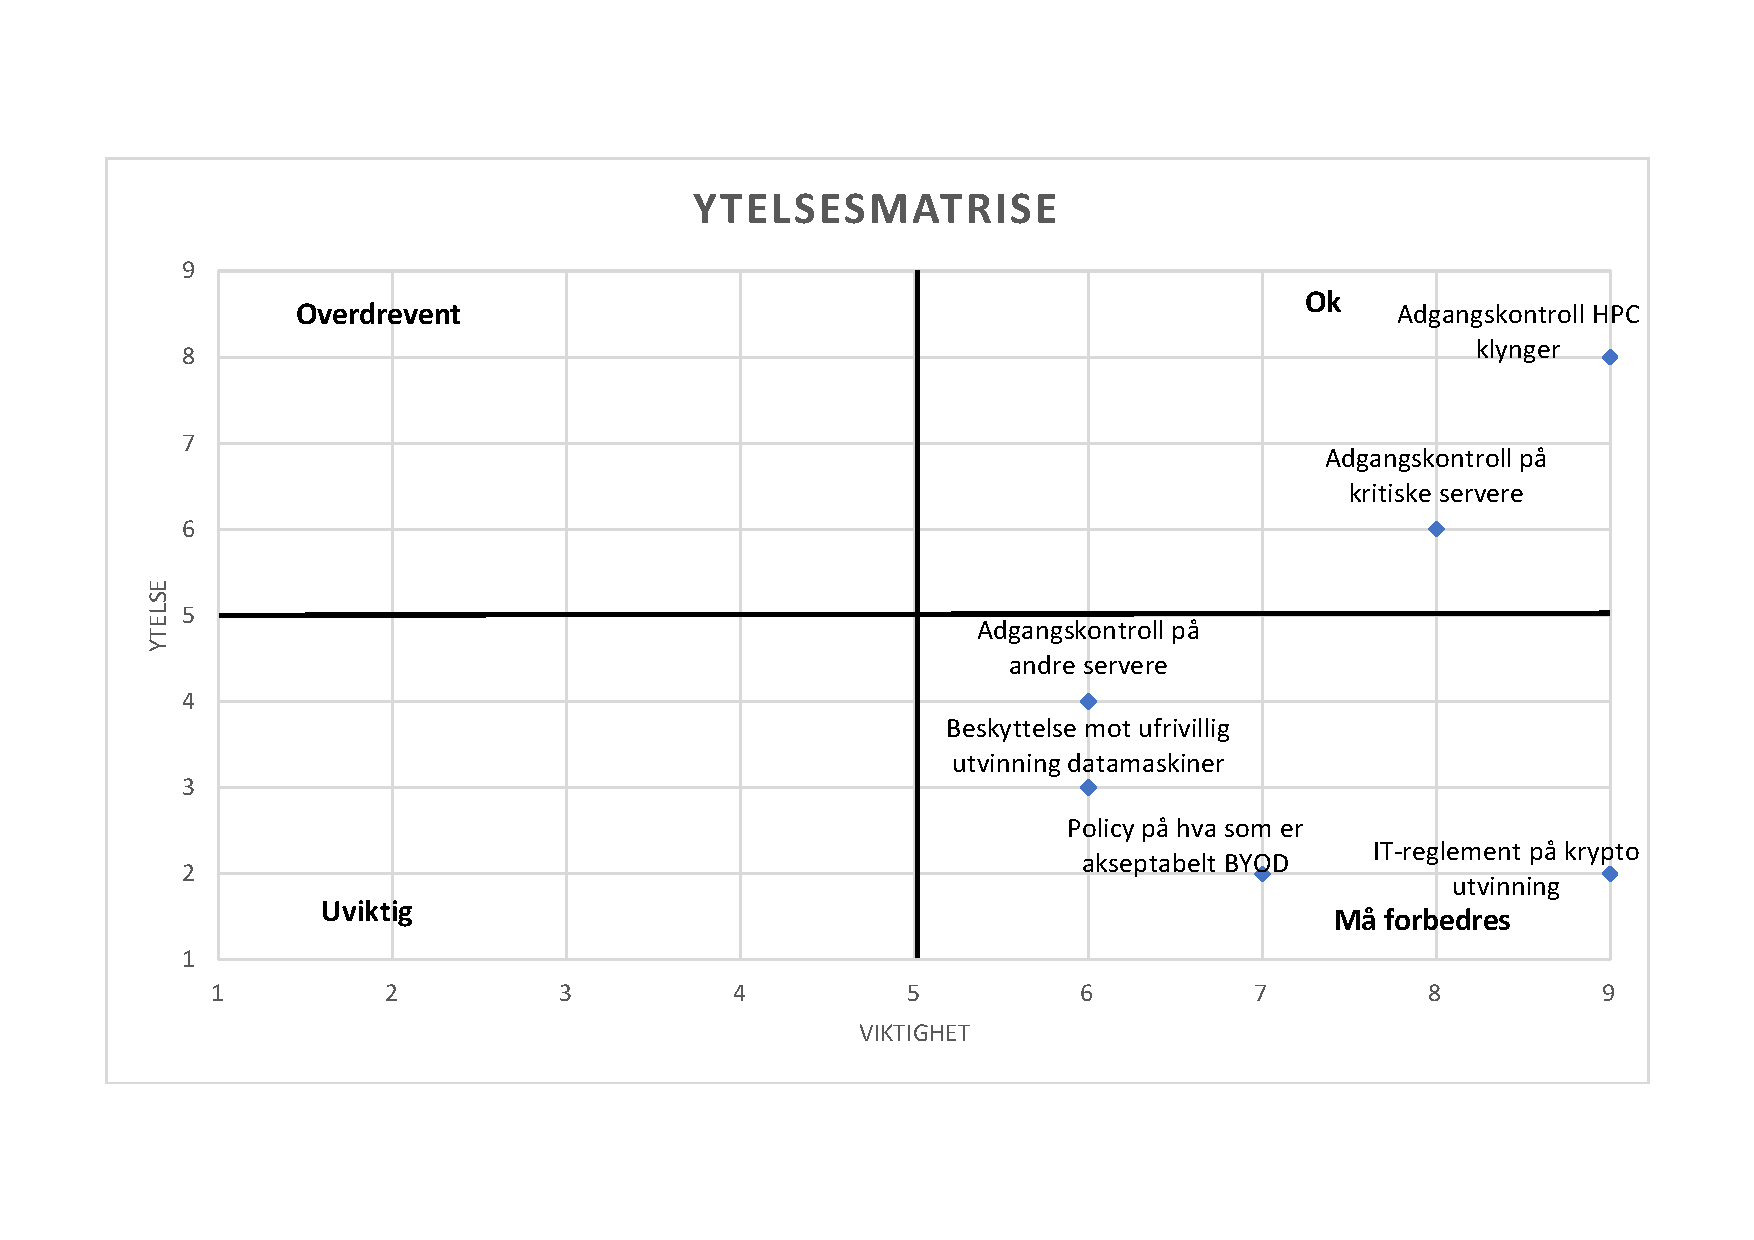
\includegraphics[scale=0.5]{case_3/bilder/ytelsesmatrise.pdf}
    \caption[Ytelsesmatrise]{Resultater fra ytelsesmatrisen}
    \label{fig:ytelsesmatrise}
\end{figure}
Det er mest kritisk å vurdere de aktiva som havner under ``må forbedres''. Selv om noen aktiva havner under ``ok'', bør de fortsatt vurderes, men de vil ha lavere prioritet enn de nevnt over. Aktiva som er uviktig eller overdrevent trenger man ikke vurdere nøye. Matrisen viser følgende prioriteringsgrunnlag til utbedring:

\begin{enumerate}
    \item Datamaskiner
    \item Andre servere
    \item Kritiske servere
    \item HPC klynger
\end{enumerate}

\subsection{Konklusjon av verktøyet}
Verktøyet var nyttig for å finne frem til et prioritetsgrunnlag for de ulike enhetene som kan misbrukes eller misbruke NTNU sine ressurser. Vi ser at det er vanlige datamaskiner som utgjør den største trusselen for misbruk. 